%-- Intro --%

\begin{tframe}{Introduction}

\vspace{0.5cm}
Digital images are easy to manipulate thanks to the availability of the \textbf{powerful editing software} and \textbf{sophisticated digital cameras}.

\vspace{1cm}


\begin{minipage}{\textwidth}
\begin{columns}[T]
\begin{column}{0.5\textwidth}
\vspace{0.1cm}
The development of methods for verifying \textbf{image authenticity} is a real need in forensics.

\vspace{0.8cm}
\textbf{Purpose}: to detect image splicing  aimed at \emph{deceiving} the viewer.
\end{column}
\begin{column}{0.4\textwidth}

\includegraphics[width=0.8\textwidth]{images/image-editing.jpg}
\end{column}
\end{columns}
\end{minipage}

\end{tframe}

%-- Image compositions --%

\begin{tframe}{Forgery detection}
\vspace{0.2cm}
Image splicing detection techniques are based on \textit{inconsistencies}:
\vspace{0.3cm}
\begin{enumerate}
\item \textbf{Image resampling, copy-paste}: deduced from image metadata.
\vspace{0.3cm}

\item \textbf{Compression-based inconsistencies}: JPEG compression introduces blocking artifacts. Manufacturers of digital cameras and image processing software typically use different JPEG quantization tables.
\vspace{0.3cm}

\item  \textbf{Neighboring pixels relationship inconsistencies}: when an image is spliced some artifacts can be created.
\vspace{0.3cm}
\item \textbf{Intrinsic image properties inconsistencies}: e.g. scene lights, shadows or perspective.
\end{enumerate}

\end{tframe}

%-- Light based detection --%

\begin{tframe}{Lighting-based inconsistencies}
\vspace{0.2cm}
Methods based on \textbf{Lighting inconsistencies} are particularly \emph{robus}: a perfect illumination adjustment in a image composition is very hard to achieve.
\vspace{0.3cm}
\begin{center}
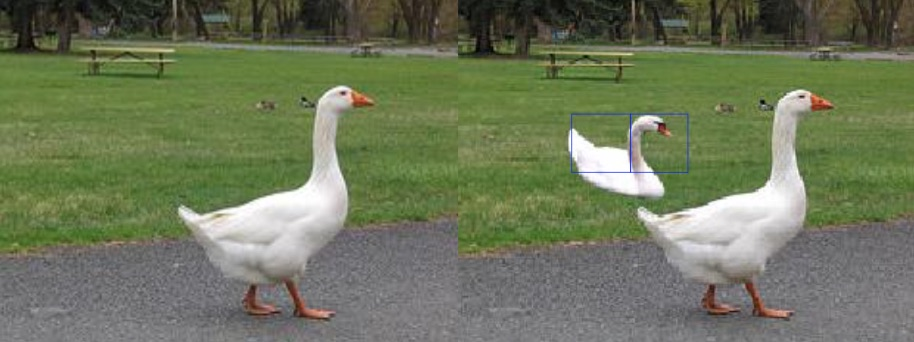
\includegraphics[width=0.5\textwidth]{images/ducks.jpg}
\vspace{0.1cm}
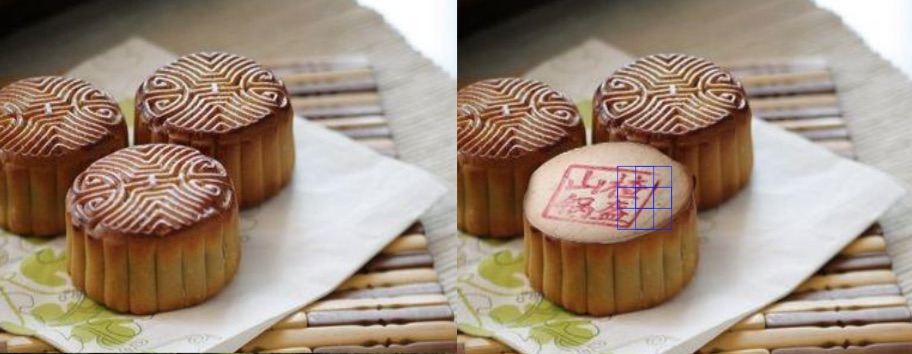
\includegraphics[width=0.5\textwidth]{images/cakes.jpg}
\end{center}
\end{tframe}

\begin{tframe}{Lighting-based inconsistencies}
\vspace{0.1cm}
These methods can be divided into two types of approaches:
\vspace{0.2cm}
\begin{enumerate}
\item \textbf{Object light source inconsistencies}: detected using \emph{shadows}, \emph{face geometry}, \emph{generic object surfaces}.
\vspace{0.2cm}

\item \textbf{Illuminant colors inconsistencies}: {\small assuming that a scene is lit by the same light source, all objects must have the same illuminant colors.}
\vspace{0.2cm}
\begin{enumerate}
\item \textit{Specular dichromatic reflectance models}
\vspace{0.1cm}
\item \textit{Illuminant Maps (IMs)}
\end{enumerate}
\end{enumerate}
\begin{center}
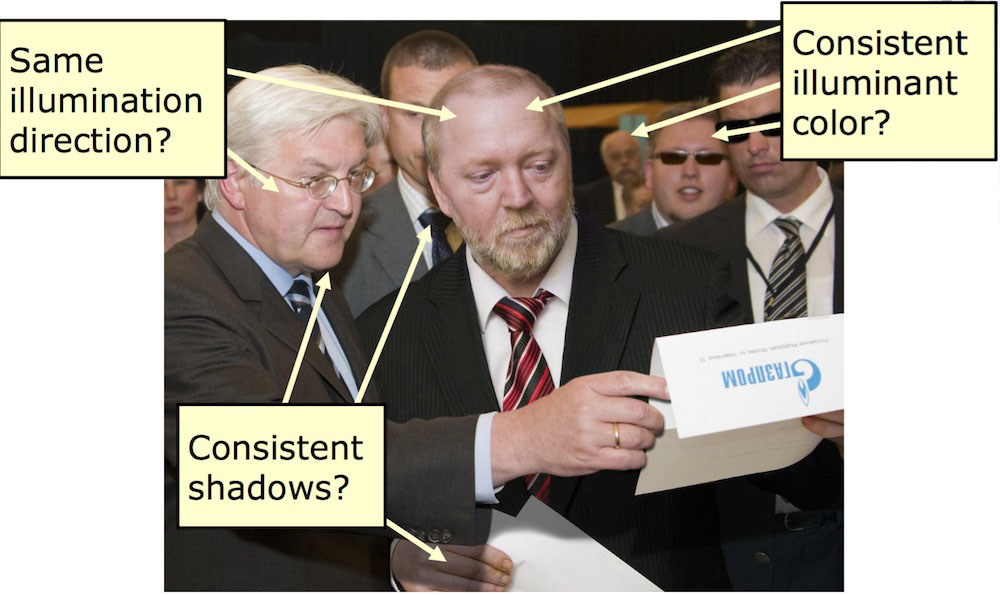
\includegraphics[width=0.4\textwidth]{images/lighting-based.jpg}
\end{center}
\end{tframe}

\begin{tframe}{Spectral dichromatic reflectance models\\{\small [Gholap and Bora 08]}}
\vspace{0.1cm}
Reflection of any materials can be modelled as additive mixture of two components: \textbf{diffused reflection}. $L_B(\lambda)$, and \textbf{surface reflection}, $L_S(\lambda)$. So, the \emph{reflected light} can be written as:
$$L(\Theta, \lambda) = m_S(\Theta)* L_S(\lambda) + m_B(\Theta) * L_B(\lambda)$$

\begin{center}
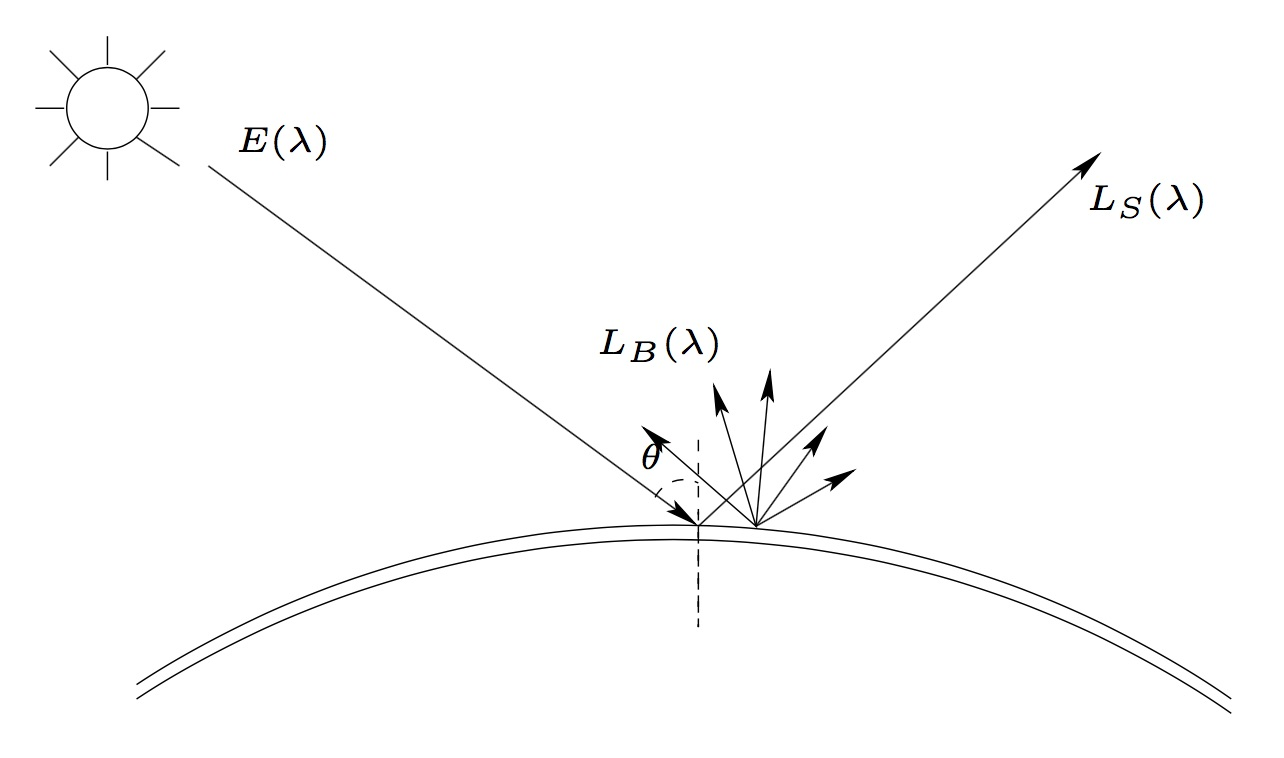
\includegraphics[width=0.4\textwidth]{images/reflectance.jpg}
\end{center}

The two vectors $L_B(\lambda)$ and $L_S(\lambda)$ span the two dimensional plane called \textbf{dichromatic plane}.
\end{tframe}


\begin{tframe}{Spectral dichromatic reflectance models\\{\small [Gholap and Bora 08]}}
\vspace{0.1cm}
\begin{minipage}{\textwidth}
\begin{columns}[T]
\begin{column}{0.5\textwidth}
\vspace{0.4cm}
From the two \emph{dichromatic plane}, the \textbf{dichromatic line} is estimated: given two dichromatic lines of different objects, they intersects at a point giving the chromaticity values of the illuminant color. 

\vspace{1.1cm}

\textbf{Detection}: if a object is spliced into the image, ad error is introduced in the estimation.
\end{column}
\begin{column}{0.4\textwidth}
\centering
\vspace{1cm}

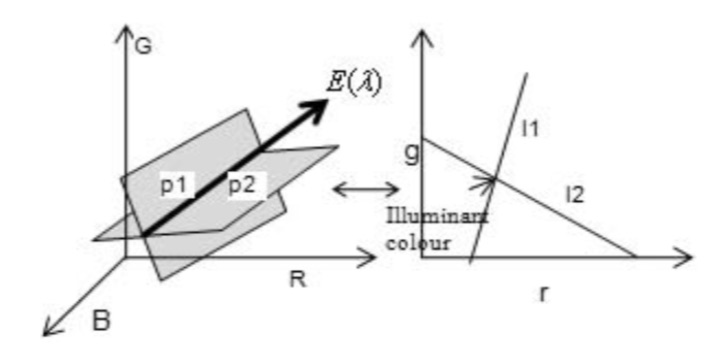
\includegraphics[width=\textwidth]{images/dichromatic-plane.jpg}
\end{column}
\end{columns}
\end{minipage}

\end{tframe}



